\documentclass[bwprint]{gmcmthesis}
\usepackage{amsmath}
\setlength{\emergencystretch}{2em}
\setkeys{Gin}{width=.9\linewidth,height=.65\textheight,keepaspectratio}
\numberwithin{figure}{section}
\renewcommand{\thefigure}{\thesection-\arabic{figure}}
\numberwithin{table}{section}
\renewcommand{\thetable}{\thesection-\arabic{table}}
\numberwithin{equation}{section}
\newcolumntype{Y}{>{\raggedright\arraybackslash}X}
\newcommand{\figref}[1]{图~\ref{#1}}
\newcommand{\tabref}[1]{表~\ref{#1}}
\newcommand{\eqnref}[1]{式~\eqref{#1}}

% 将以下占位信息替换为自己的信息。
\title{数学建模论文标题（模板示例）}
\baominghao{00000000000}
\schoolname{学校名称}
\membera{成员一}
\memberb{成员二}
\memberc{成员三}

\begin{document}
\maketitle
\begin{abstract}
本文为数学建模论文的排版模板。摘要通常介绍研究问题、建模方法、主要结果与结论，请在使用时替换为自己的内容。本模板演示章节组织、数学公式、图片引用、三线表、可跨页长表以及参考文献。所有数值表格均为虚构排版示例；示例图片仅用于展示插图方式，不构成本文的研究结果。
\keywords{数学建模；LaTeX；公式；图片；跨页表格}
\end{abstract}
\tableofcontents
\clearpage

\section{问题重述}
在这里介绍问题背景、研究目标及需要解决的子问题。可以使用\verb|\section|、\verb|\subsection|组织内容，使用\verb|\label|和\verb|\ref|建立交叉引用。
\subsection{问题分析}
说明输入数据、输出目标与模型的适用范围。使用文献时，在相应论述处引用，例如排版方法可参考文献\cite{latex-book}。

\section{模型假设与符号说明}
\begin{enumerate}
\item 假设输入数据已完成必要的整理。
\item 假设模型参数在所讨论区间内保持不变。
\item 上述内容仅为模板占位，应按实际问题修改。
\end{enumerate}
\begin{table}[htbp]
\centering
\caption{符号说明示例}\label{tab:symbols}
\begin{tabularx}{.85\linewidth}{cYc}
\toprule
符号 & 含义 & 单位 \\
\midrule
$x_i$ & 第 $i$ 个输入变量 & 无量纲 \\
$y_i$ & 第 $i$ 个观测值 & 无量纲 \\
$n$ & 样本数量 & 个 \\
\bottomrule
\end{tabularx}
\end{table}

\section{数学公式示例}
\subsection{行内公式与编号公式}
行内公式示例为 $a^2+b^2=c^2$。下面的均方误差可通过\eqnref{eq:mse}引用：
\begin{equation}
\operatorname{MSE}=\frac{1}{n}\sum_{i=1}^{n}(y_i-\hat y_i)^2.
\label{eq:mse}
\end{equation}
\subsection{多行公式、矩阵与分段函数}
\begin{align}
\hat y_i &= \beta_0+\beta_1 x_i,\\
\hat{\boldsymbol\beta} &= \arg\min_{\boldsymbol\beta}
\sum_{i=1}^{n}(y_i-\beta_0-\beta_1x_i)^2.
\end{align}
\begin{equation}
A=\begin{pmatrix}1&2\\3&4\end{pmatrix},\qquad
f(x)=\begin{cases}x^2,&x\geq0,\\-x,&x<0.\end{cases}
\end{equation}
\begin{equation}
\int_0^1 x^2\,\mathrm{d}x=\frac13.
\end{equation}

\section{图片示例与格式说明}
\subsection{插图和交叉引用}
图片放在\path{figures/}目录，通过\verb|\includegraphics|插入。图题应说明图片表达的内容；使用\verb|\label|后，可像\figref{fig:example}这样引用。
\begin{figure}[htbp]
\centering
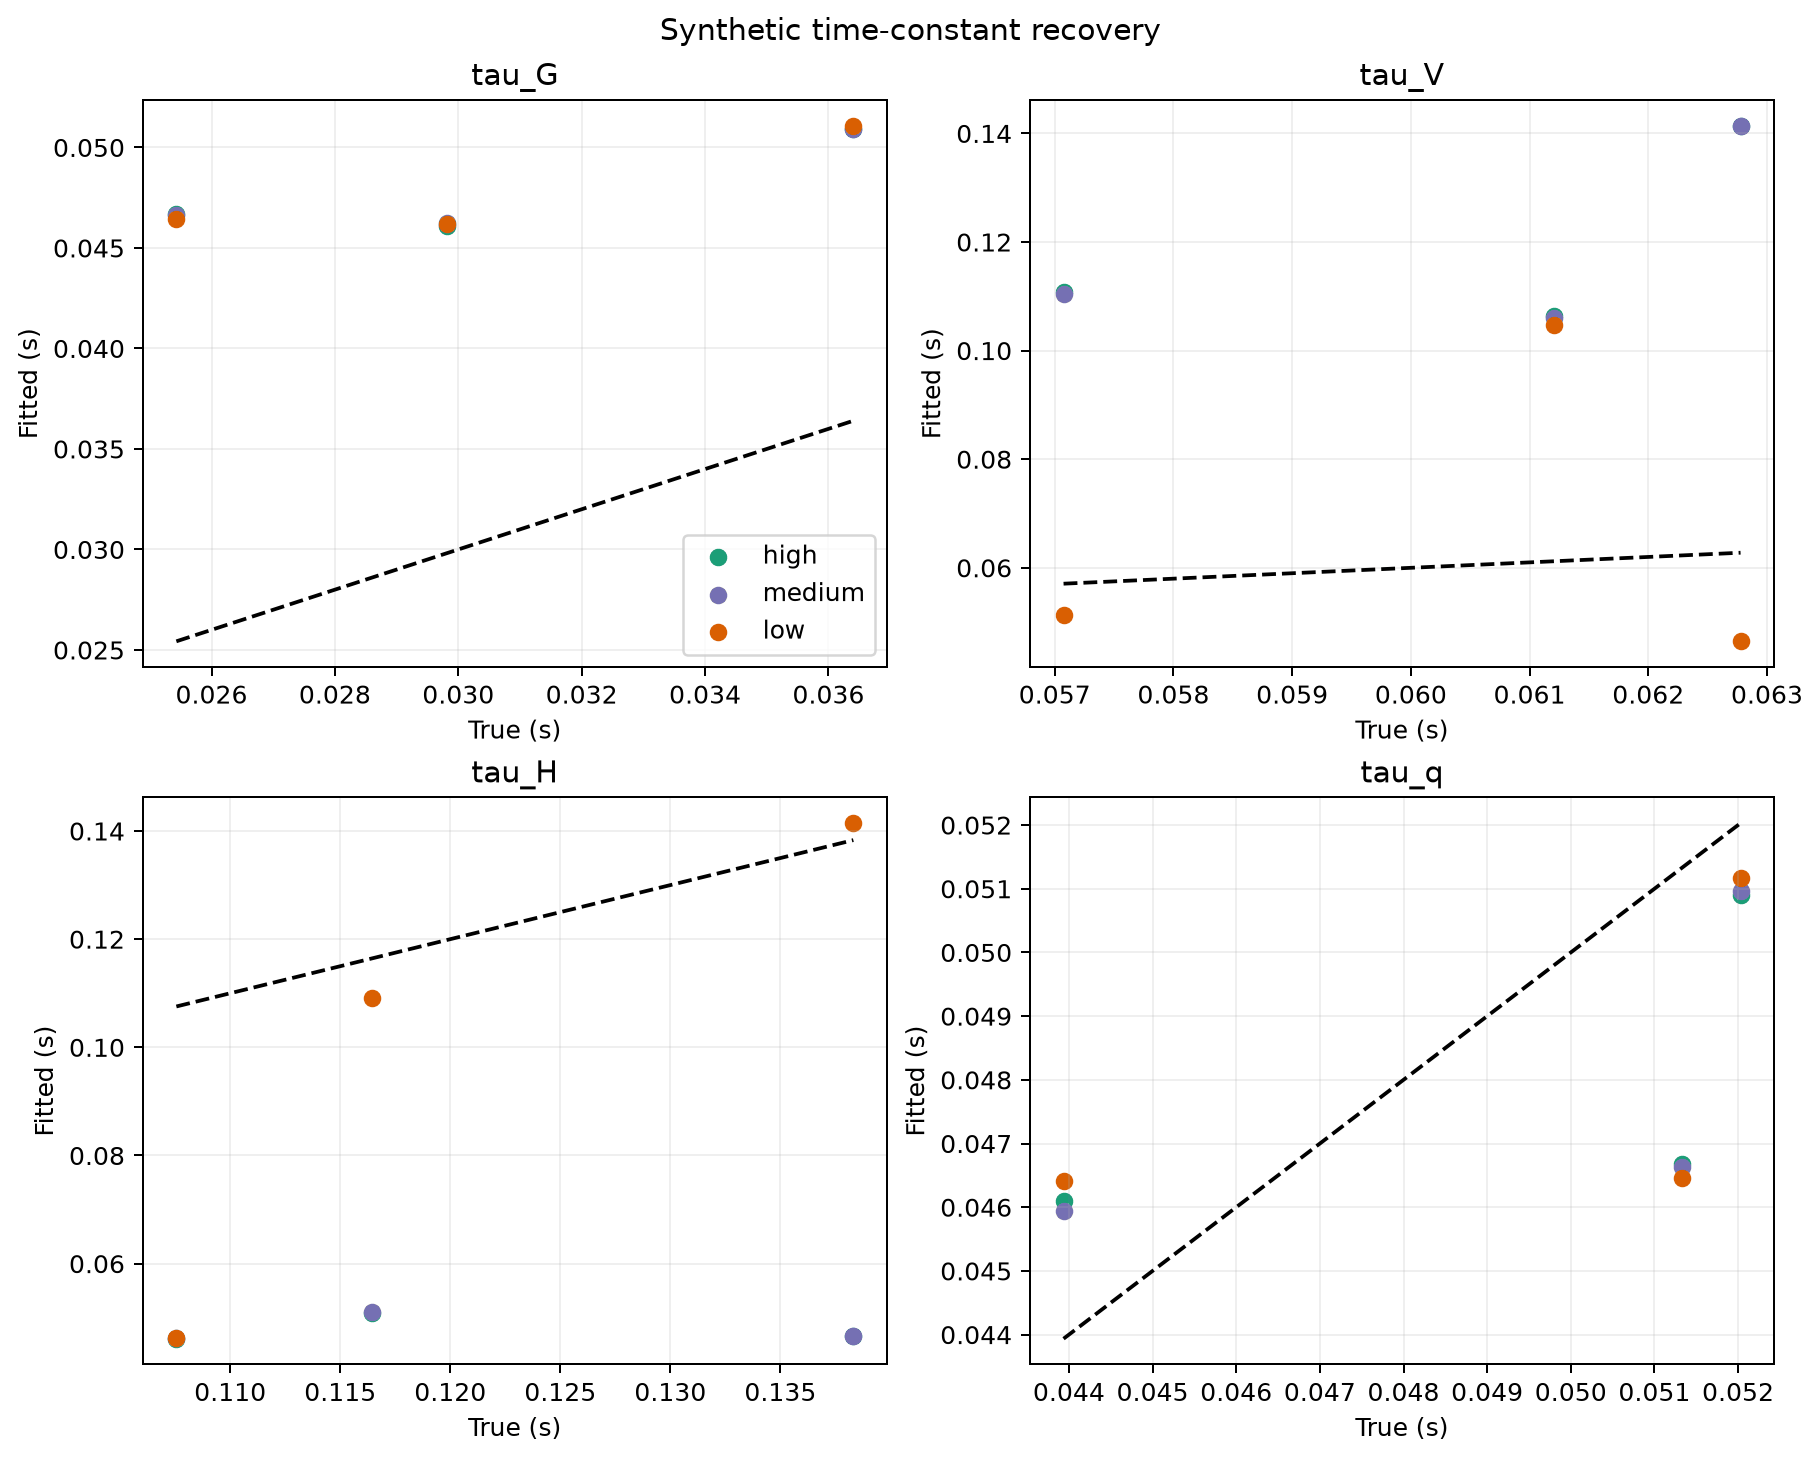
\includegraphics[width=.8\linewidth]{figures/figures__q2_model_a__06_parameter_recovery.png}
\caption{现有图片的排版示例（仅演示图片尺寸、图题和引用）}
\label{fig:example}
\end{figure}
\begin{figure}[htbp]
\centering
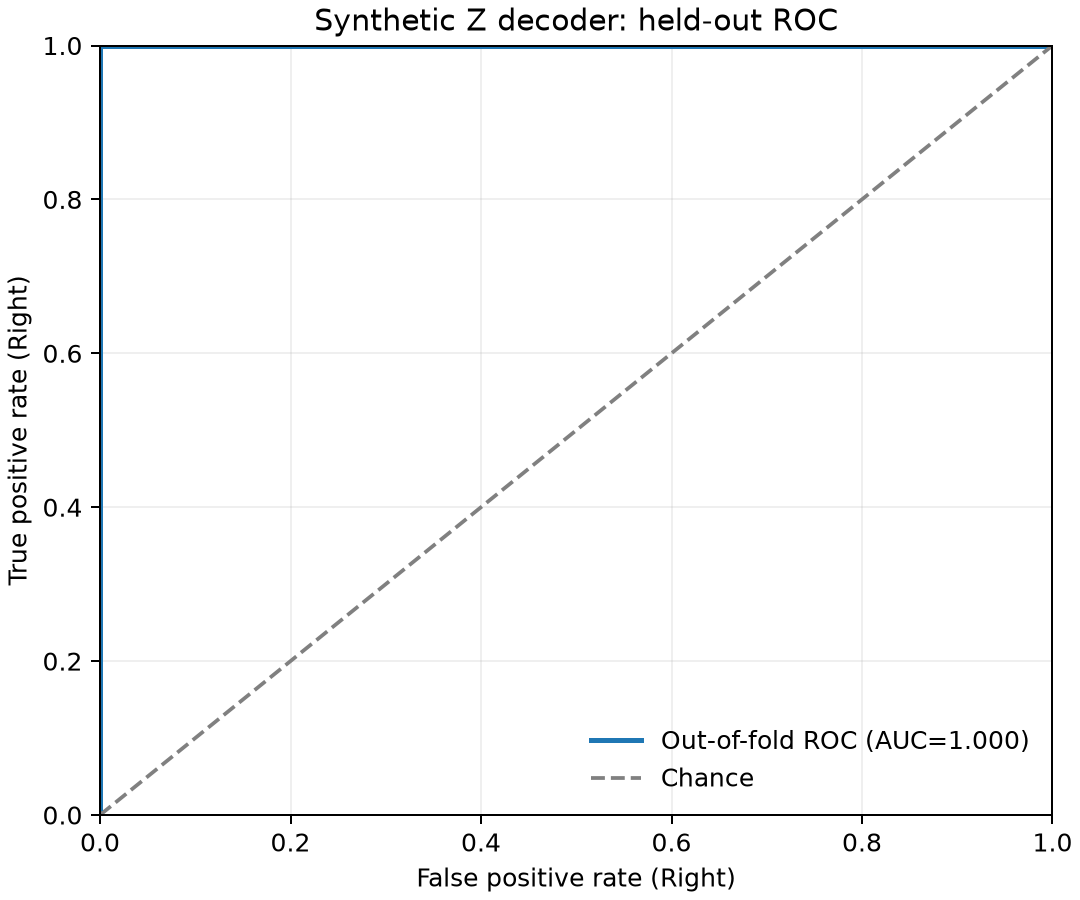
\includegraphics[width=.75\linewidth]{figures/figures__synthetic_z_decoder__balanced_100_each_noise_0p01_seed_20260926__roc_curve.png}
\caption{曲线图排版示例（沿用图片内容，不作研究结论）}
\label{fig:curve}
\end{figure}

\subsection{图片格式选择}
\tabref{tab:formats}列出常用图片格式。PDF 的矢量部分放大不失真；如果 PDF 中嵌入位图，该部分仍受像素分辨率限制。PNG 适合热图、照片和像素图；LaTeX 通常需要先将 SVG 转为 PDF 再引用。
\begin{table}[htbp]
\centering\small
\caption{图片格式与推荐用途}\label{tab:formats}
\begin{tabularx}{\linewidth}{@{}l l l Y l Y@{}}
\toprule
格式 & 类型 & 放大是否失真 & LaTeX 支持 & 文件大小 & 推荐用途 \\
\midrule
\textbf{PDF} & vector & 不失真 & \textbf{原生支持，非常好} & 通常较小 & \textbf{论文作图首选} \\
PNG & raster & 会失真 & 原生支持 & 可能较大 & heatmap、照片、像素图 \\
SVG & vector & 不失真 & 非原生，需要转换 & 通常较小 & 网页、Inkscape 编辑、中间文件 \\
\bottomrule
\end{tabularx}
\end{table}
\begin{lstlisting}[language=TeX]
% Replace with an existing file. PDF and PNG use the same command.
\includegraphics[width=0.8\linewidth]{figures/example.pdf}
\includegraphics[width=0.8\linewidth]{figures/example.png}
\end{lstlisting}
上述文件名为说明用占位路径，不参与编译。转换 SVG 时，可以使用 Inkscape 导出 PDF，再按上述方式引用。
\clearpage

\section{可跨页三线表示例}
\label{sec:longtable}
下表使用\verb|longtable|环境，直接放在正文中，无须外套\verb|table|浮动环境。它会自动跨页。

\verb|\endfirsthead|定义首页表头，\verb|\endhead|定义续页表头。

\verb|\endfoot|定义普通页脚，\verb|\endlastfoot|定义末页页脚。表中的数值是虚构示例。
\begingroup
\small
\setlength{\tabcolsep}{6pt}
\renewcommand{\arraystretch}{1.25}
\begin{longtable}{@{}r p{.28\linewidth} r r p{.24\linewidth}@{}}
\caption{虚构数据的可跨页三线表示例}\label{tab:long-example}\\
\toprule
序号 & 样本名称 & 输入值 & 输出值 & 备注 \\
\midrule
\endfirsthead
\caption[]{虚构数据的可跨页三线表示例（续）}\\
\toprule
序号 & 样本名称 & 输入值 & 输出值 & 备注 \\
\midrule
\endhead
\midrule
\multicolumn{5}{r}{续下页}\\
\endfoot
\bottomrule
\endlastfoot
1 & 示例样本 01 & 0.1 & 1.2 & 虚构排版数据 \\
2 & 示例样本 02 & 0.2 & 1.4 & 虚构排版数据 \\
3 & 示例样本 03 & 0.3 & 1.6 & 虚构排版数据 \\
4 & 示例样本 04 & 0.4 & 1.8 & 虚构排版数据 \\
5 & 示例样本 05 & 0.5 & 2.0 & 虚构排版数据 \\
6 & 示例样本 06 & 0.6 & 2.2 & 虚构排版数据 \\
7 & 示例样本 07 & 0.7 & 2.4 & 虚构排版数据 \\
8 & 示例样本 08 & 0.8 & 2.6 & 虚构排版数据 \\
9 & 示例样本 09 & 0.9 & 2.8 & 虚构排版数据 \\
10 & 示例样本 10 & 1.0 & 3.0 & 虚构排版数据 \\
11 & 示例样本 11 & 1.1 & 3.2 & 虚构排版数据 \\
12 & 示例样本 12 & 1.2 & 3.4 & 虚构排版数据 \\
13 & 示例样本 13 & 1.3 & 3.6 & 虚构排版数据 \\
14 & 示例样本 14 & 1.4 & 3.8 & 虚构排版数据 \\
15 & 示例样本 15 & 1.5 & 4.0 & 虚构排版数据 \\
16 & 示例样本 16 & 1.6 & 4.2 & 虚构排版数据 \\
17 & 示例样本 17 & 1.7 & 4.4 & 虚构排版数据 \\
18 & 示例样本 18 & 1.8 & 4.6 & 虚构排版数据 \\
19 & 示例样本 19 & 1.9 & 4.8 & 虚构排版数据 \\
20 & 示例样本 20 & 2.0 & 5.0 & 虚构排版数据 \\
21 & 示例样本 21 & 2.1 & 5.2 & 虚构排版数据 \\
22 & 示例样本 22 & 2.2 & 5.4 & 虚构排版数据 \\
23 & 示例样本 23 & 2.3 & 5.6 & 虚构排版数据 \\
24 & 示例样本 24 & 2.4 & 5.8 & 虚构排版数据 \\
25 & 示例样本 25 & 2.5 & 6.0 & 虚构排版数据 \\
26 & 示例样本 26 & 2.6 & 6.2 & 虚构排版数据 \\
27 & 示例样本 27 & 2.7 & 6.4 & 虚构排版数据 \\
28 & 示例样本 28 & 2.8 & 6.6 & 虚构排版数据 \\
29 & 示例样本 29 & 2.9 & 6.8 & 虚构排版数据 \\
30 & 示例样本 30 & 3.0 & 7.0 & 虚构排版数据 \\
31 & 示例样本 31 & 3.1 & 7.2 & 虚构排版数据 \\
32 & 示例样本 32 & 3.2 & 7.4 & 虚构排版数据 \\
33 & 示例样本 33 & 3.3 & 7.6 & 虚构排版数据 \\
34 & 示例样本 34 & 3.4 & 7.8 & 虚构排版数据 \\
35 & 示例样本 35 & 3.5 & 8.0 & 虚构排版数据 \\
36 & 示例样本 36 & 3.6 & 8.2 & 虚构排版数据 \\
37 & 示例样本 37 & 3.7 & 8.4 & 虚构排版数据 \\
38 & 示例样本 38 & 3.8 & 8.6 & 虚构排版数据 \\
39 & 示例样本 39 & 3.9 & 8.8 & 虚构排版数据 \\
40 & 示例样本 40 & 4.0 & 9.0 & 虚构排版数据 \\
41 & 示例样本 41 & 4.1 & 9.2 & 虚构排版数据 \\
42 & 示例样本 42 & 4.2 & 9.4 & 虚构排版数据 \\
43 & 示例样本 43 & 4.3 & 9.6 & 虚构排版数据 \\
44 & 示例样本 44 & 4.4 & 9.8 & 虚构排版数据 \\
45 & 示例样本 45 & 4.5 & 10.0 & 虚构排版数据 \\
46 & 示例样本 46 & 4.6 & 10.2 & 虚构排版数据 \\
47 & 示例样本 47 & 4.7 & 10.4 & 虚构排版数据 \\
48 & 示例样本 48 & 4.8 & 10.6 & 虚构排版数据 \\
49 & 示例样本 49 & 4.9 & 10.8 & 虚构排版数据 \\
50 & 示例样本 50 & 5.0 & 11.0 & 虚构排版数据 \\
51 & 示例样本 51 & 5.1 & 11.2 & 虚构排版数据 \\
52 & 示例样本 52 & 5.2 & 11.4 & 虚构排版数据 \\
53 & 示例样本 53 & 5.3 & 11.6 & 虚构排版数据 \\
54 & 示例样本 54 & 5.4 & 11.8 & 虚构排版数据 \\
55 & 示例样本 55 & 5.5 & 12.0 & 虚构排版数据 \\
56 & 示例样本 56 & 5.6 & 12.2 & 虚构排版数据 \\
57 & 示例样本 57 & 5.7 & 12.4 & 虚构排版数据 \\
58 & 示例样本 58 & 5.8 & 12.6 & 虚构排版数据 \\
59 & 示例样本 59 & 5.9 & 12.8 & 虚构排版数据 \\
60 & 示例样本 60 & 6.0 & 13.0 & 虚构排版数据 \\
\end{longtable}
\endgroup
\tabref{tab:long-example}展示了跨页后的表头与页脚。避免使用\verb|\resizebox|包裹长表，否则无法正常跨页。

\section{结果分析与总结}
在这里填写模型结果、误差分析、优点、局限与后续工作。请将占位段落、虚构数据及示例图片替换为自己的内容。

\begin{thebibliography}{9}
\bibitem{latex-book} Leslie Lamport. \emph{LaTeX: A Document Preparation System}. 2nd ed. Addison-Wesley, 1994.
\end{thebibliography}

\appendix
\section{编译说明}
本模板使用 XeLaTeX。通常连续编译两次，以更新目录与交叉引用：
\begin{lstlisting}[language=bash]
xelatex -interaction=nonstopmode -halt-on-error main.tex
xelatex -interaction=nonstopmode -halt-on-error main.tex
\end{lstlisting}
项目地址：\url{https://github.com/713s/gmcm-latex-template}。
\end{document}
